\documentclass[english,t]{beamer}
%\documentclass[handout,english]{beamer}

\mode<presentation>
{
  \usetheme{Copenhagen}
  % oder ...
  
%  \setbeamercovered{transparent}
  % oder auch nicht
}

%\usepackage[pdftex]{graphicx}
\graphicspath{{/home/ave/doc/images/}{}{../teranaloppu/}{../metodi/}{../slides/Hartikainen/}{../gphealth/}{../2008_09_RSS2008/}{../gphealth/}{../jyvaskyla2009/}{../nbbc2009/}{../gphealth/hippics/}{../euroheis2010/}{../pubgensens2011/}{../reykjavik2013/}{../liverpool2013/}{../../gpstuff/doc/}{./images/}{../aalto_stochastic/}{figs/}{../Stancon2018Helsinki/figs/}{../../paper/cvapprox/}{../gppa2017/}{../valencia2017/}{../../paper/combine_predictive_distribution/tex/}{../venice2018/figs/}{./figs/}{../slides/figs/}}
\usepackage[T1]{fontenc}
\usepackage[utf8]{inputenc}
\usepackage{times}
\usepackage{amsmath,amsfonts,amssymb}
%\usepackage{euscript}
\usepackage{afterpage}
%\usepackage{picinpar}
%\usepackage{array,longtable}
\usepackage{url}
\urlstyle{same}
%\usepackage{eufrak}
\usepackage{amsbsy}
\usepackage{eucal}
\usepackage{rotating}
\usepackage{bm}
\usepackage{pdfpages}
\usepackage{algorithm}
\usepackage[noend]{algpseudocode}
\usepackage{booktabs}
\usepackage{listings}
\usepackage{lstbayes}
\usepackage{microtype}

\usepackage{natbib}
\bibliographystyle{apalike}

\hypersetup{%
  bookmarksopen=true,
  bookmarksnumbered=true,
  pdftitle={Stan},
  pdfsubject={Bayesian data analysis},
  pdfauthor={Aki Vehtari},
  pdfkeywords={},
  pdfstartview={FitH -32768},
  colorlinks=true,
  linkcolor=navyblue,
  citecolor=navyblue,
  filecolor=navyblue,
  urlcolor=navyblue
}

%%%%%%%%%%%%%%%%%%% for tikz figures %%%%%%%%%%%%%%%%%%%%%%%%%%
\usepackage{ifthen}
\usepackage{tikz,pgfplots}
\usetikzlibrary{matrix}
\usetikzlibrary{calc}
\newlength{\figurewidth}
\newlength{\figureheight}


\def\figpdfdir{./fig/} % directory for pdf-figures
\def\figtikzdir{./tikz/} % directory for tikz-figures 

% this is replacement for the \input command used in the figure-environment which
% takes into account whether pdf is forced
\newcommand{\minput}[2][]{
\ifthenelse{\equal{#1}{pdf}}
	{ \includegraphics{\figpdfdir #2} }
	{ \tikzset{external/remake next} \tikzsetnextfilename{#2} \input{\figtikzdir #2} }
}

% for externalization
\usetikzlibrary{external}
\tikzexternalize[prefix=\figpdfdir] 
\tikzset{external/system call={lualatex
	\tikzexternalcheckshellescape -halt-on-error -interaction=batchmode
	-jobname "\image" "\texsource"}}
    
%%%%%%%%%%%%%%%%%%% for hiding figures %%%%%%%%%%%%%%%%%%%%%%%%%%
\usepackage{color}
\newcommand{\hide}[5][white]{
	% usage: \hhide[color]{vspace,hspace,height,width}
	% note: all measures are relative units measured in \textwidth
	%\begin{minipage}{0.99\textwidth}
	\vspace{#2\textwidth}
	\hspace{#3\textwidth}
	\textcolor{#1}{  \rule{#5\textwidth}{#4\textwidth}  }
	% \end{minipage}
      }

\DeclareMathOperator{\Kfu}{\mathbf{K}_{f,u}}
\DeclareMathOperator{\Kuf}{\mathbf{K}_{u,f}}
\DeclareMathOperator{\Kff}{\mathbf{K}_{f,f}}
\DeclareMathOperator{\iKff}{\mathbf{K}_{f,f}^{-1}}
\DeclareMathOperator{\Kfa}{\mathbf{K}_{f,\tilde{f}}}
\DeclareMathOperator{\Kaf}{\mathbf{K}_{\tilde{f},f}}
\DeclareMathOperator{\Kaa}{\mathbf{K}_{\tilde{f},\tilde{f}}}
\DeclareMathOperator{\Kuu}{\mathbf{K}_{u,u}}
\DeclareMathOperator{\iKuu}{\mathbf{K}_{u,u}^{-1}}
\DeclareMathOperator{\Kau}{\mathbf{K}_{\tilde{f},u}}
\DeclareMathOperator{\Kua}{\mathbf{K}_{u,\tilde{f}}}
\DeclareMathOperator{\Qff}{\mathbf{Q}_{f,f}}
\DeclareMathOperator{\Qaa}{\mathbf{Q}_{\tilde{f},\tilde{f}}}
\DeclareMathOperator{\Qfa}{\mathbf{Q}_{f,\tilde{f}}}
\DeclareMathOperator{\Qaf}{\mathbf{Q}_{\tilde{f},f}}
\DeclareMathOperator{\x}{\mathbf{x}}
\DeclareMathOperator{\f}{\mathbf{f}}
\DeclareMathOperator{\y}{\mathbf{y}}
\DeclareMathOperator{\h}{\mathbf{h}}
\DeclareMathOperator{\uu}{\mathbf{u}}
\DeclareMathOperator{\LL}{\mathbf{\Lambda}}
\DeclareMathOperator{\bb}{\mathbf{b}}
\DeclareMathOperator{\E}{\mathrm{E}}
\def\WAIC{\mathrm{WAIC}}

\newcommand{\kin}{k^{\rm in}}
\newcommand{\kout}{k^{\rm out}}
\newcommand{\gi}{{R_0}}
\newcommand{\eff}{{E_{\rm max}}}
\newcommand{\HN}{{\rm N^+}}
\newcommand{\lN}{{\rm LN}}
\newcommand{\Rss}{R^{\rm ss}}
\newcommand{\invlogit}{\mbox{logit}^{-1}}
\newcommand{\KLx}[2] { \mathrm{KL} {\left(#1 \, \| \, #2\right)} }
\newcommand{\vs}[1] { \boldsymbol{#1} }
% \DeclareMathOperator{\Poisson}{Poisson}
\DeclareMathOperator{\Chi}{Chi}
\DeclareMathOperator{\GP}{\mathcal{GP}}
%\DeclareMathOperator{\N}{N}
\DeclareMathOperator{\KL}{KL}

\DeclareMathOperator*{\argmax}{arg\,max}
\DeclareMathOperator*{\argmin}{arg\,min}
\newcommand{\mb}{\mathbf}
\newcommand{\pkg}[1]{{\fontseries{b}\selectfont #1}}
\newcommand{\proglang}{}
\newcommand{\email}[1]{\href{mailto:#1}{\normalfont\texttt{#1}}}
\newcommand{\doi}[1]{\href{http://dx.doi.org/#1}{\normalfont\texttt{doi:#1}}}
\newcommand{\code}[1]{{\normalfont\texttt{#1}}}

% \DeclareMathOperator{\E}{E}
% \DeclareMathOperator{\VAR}{Var}
% \DeclareMathOperator{\COV}{Cov}
% \DeclareMathOperator{\Prob}{P}
% \DeclareMathOperator{\E}{E}
\DeclareMathOperator{\Var}{Var}
\DeclareMathOperator{\var}{var}
\DeclareMathOperator{\cov}{cov}
\DeclareMathOperator{\logistic}{logistic}
\DeclareMathOperator{\softmax}{softmax}
\DeclareMathOperator{\Multinomial}{Multinomial}
\DeclareMathOperator{\Sd}{Sd}
\DeclareMathOperator{\sd}{sd}
\DeclareMathOperator{\Bin}{Bin}
\DeclareMathOperator{\Poisson}{Poisson}
\DeclareMathOperator{\Beta}{Beta}
\DeclareMathOperator{\logit}{logit}
\DeclareMathOperator{\N}{N}
\DeclareMathOperator{\U}{U}
\DeclareMathOperator{\BF}{BF}
%\DeclareMathOperator{\Pr}{Pr}
\def\euro{{\footnotesize \EUR\, }}
\DeclareMathOperator{\rep}{\mathrm{rep}}

\definecolor{set11}{HTML}{E41A1C}
\definecolor{set12}{HTML}{377EB8}
\definecolor{greenish}{rgb}{0.1333,0.8666,0.1333}
\definecolor{forestgreen}{rgb}{0.1333,0.5451,0.1333}
\definecolor{hutblue}{rgb}{0,0.2549,0.6784}
\definecolor{midnightblue}{rgb}{0.0977,0.0977,0.4375}
\definecolor{navyblue}{rgb}{0,0,0.5}
\definecolor{hutsilver}{rgb}{0.4863,0.4784,0.4784}
\definecolor{lightgray}{rgb}{0.95,0.95,0.95}
\definecolor{section}{rgb}{0,0.2549,0.6784}
\definecolor{list1}{rgb}{0,0.2549,0.6784}
\renewcommand{\emph}[1]{\textcolor{navyblue}{#1}}

%\graphicspath{./pics}

\pdfinfo{
  /Title      (Bayesian data analysis ch7)
  /Author     (Aki Vehtari) %
  /Keywords   (Bayesian probability theory, Bayesian inference, Bayesian data analysis)
}

\parindent=0pt
\parskip=8pt
\tolerance=9000
\abovedisplayshortskip=0pt

%\renewcommand{\itemsep}{0pt}
% Lists
\newenvironment{list1}{
   \begin{list}{$\color{list1}\bullet$}{\itemsep=6pt}}{
  \end{list}}
\newenvironment{list1s}{
  \begin{list}{$\includegraphics[width=5pt]{logo.eps}$}{\itemsep=6pt}}{
  \end{list}}
\newenvironment{list2}{
  \begin{list}{-}{\baselineskip=12pt\itemsep=2pt}}{
  \end{list}}
\newenvironment{list3}{
  \begin{list}{$\cdot$}{\baselineskip=15pt}}{
  \end{list}}

\setbeamertemplate{navigation symbols}{}
\setbeamertemplate{headline}[default]{}
\setbeamertemplate{headline}[text line]{\insertsection}
\setbeamertemplate{footline}[split]


\title[]{Bayesian data analysis}
\subtitle{}

\author[Aki.Vehtari@aalto.fi -- @avehtari]{Aki Vehtari}

\institute[Aalto]{}

\date[]{}

\begin{document}

\begin{frame}

  \centering

  \vskip 2\baselineskip

  \LARGE{\color{navyblue} Cost effective prediction of bodyfat}\\
      \large{\color{gray} An example of project presentation slides}


    \vskip 1\baselineskip

    \Large{Aki Vehtari}\\
    \large{Aalto University}

    \vskip 2\baselineskip

    \pause
    Introduce yourself

  
\end{frame}

\begin{frame}
  
  {\Large\color{navyblue} Measuring bodyfat percentage}


  \begin{itemize}
  \item Bodyfat percentage is related to many health outcomes
  \item<2-> Relatively accurate way to measure bodyfat is to weight a
    person in air and immersed in water
    \begin{itemize}
    \item proportion of body fat can be derived from body density with
      Siri's (1956) formula
    \item water immersion requires a big tub for the water and harness
      system for lowering a person to water
    \end{itemize}
  \item<3-> Can we estimate the bodyfat percentage with faster and a
    smaller equipment?
    \begin{itemize}
    \item with just a scale and measure tape?
    \item 252 subjects
    \end{itemize}
  \end{itemize}
  \vspace{2\baselineskip}
  \centering
  [Nice figures here]
  
\end{frame}

\begin{frame}
  
  {\Large\color{navyblue} Measuring bodyfat percentage}


  \vspace{-.5\baselineskip}
  \begin{itemize}
  \item With just a scale and measure tape?
  %   \begin{itemize}
  %   \item weight, height and circumference of different body parts
  % \end{itemize}
  \end{itemize}
  
  \vspace{-.7\baselineskip}
  \includegraphics[width=8.2cm]{bodyfat_corr.pdf}

\end{frame}


\begin{frame}
  
  {\Large\color{navyblue} Bodyfat predictive model}

  \begin{itemize}
  \item<1-> Gaussian linear regression model with normal
    vs. regularized horseshoe prior ($p_0=5$) on coefficients
  \item<2-> Model build with {\tt rstanarm} and inference run with
    Stan
    \begin{itemize}
    \item all convergence diagnostics were good
    \end{itemize}
\end{itemize}
\end{frame}

\begin{frame}
  
  {\Large\color{navyblue} Bodyfat model checking}

  Posterior predictive checking
  
  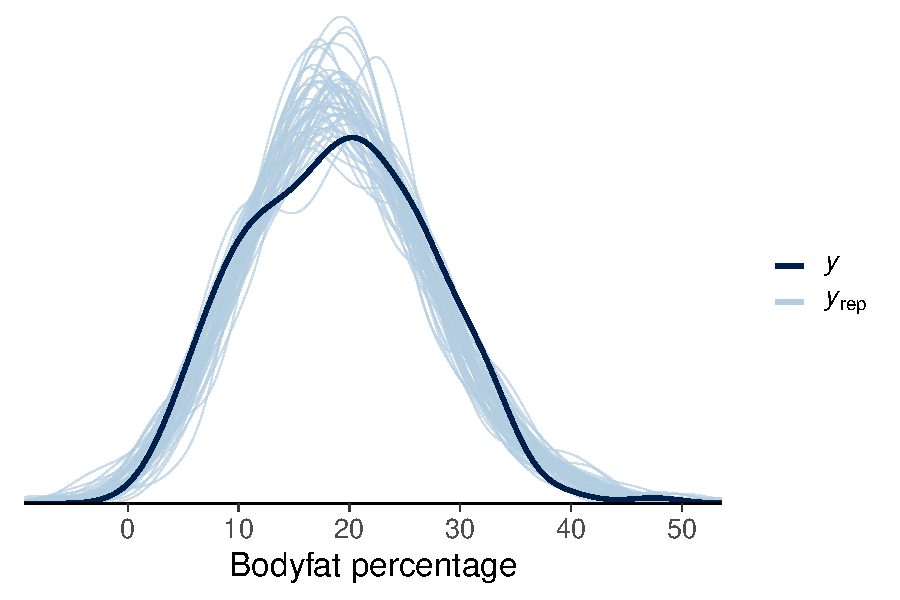
\includegraphics[width=11cm]{bodyfat_ppc.pdf}

\end{frame}

\begin{frame}[fragile]
  
  {\Large\color{navyblue} Bodyfat model comparison}

  \begin{itemize}
  \item Leave-one-out cross-validation comparison
    \begin{itemize}
    \item no difference
    \end{itemize}
    {\footnotesize
\begin{lstlisting}
               elpd_diff se_diff
RHS prior        0.0       0.0   
Gaussian prior  -1.1       2.2   
\end{lstlisting}
  }
\end{itemize}

\end{frame}

\begin{frame}[fragile]
  
  {\Large\color{navyblue} Bodyfat model comparison}

  \begin{itemize}
  \item Leave-one-out cross-validation comparison
    \begin{itemize}
    \item no difference
    \end{itemize}
    {\scriptsize
\begin{lstlisting}
               elpd_diff se_diff
RHS prior        0.0       0.0   
Gaussian prior  -1.1       2.2   
\end{lstlisting}
  }
    {\scriptsize
\begin{lstlisting}
Computed from 4000 by 250 log-likelihood matrix

         Estimate   SE
elpd_loo   -723.9  9.4
p_loo        13.4  1.2
looic      1447.9 18.8
------
Monte Carlo SE of elpd_loo is 0.1.

Pareto k diagnostic values:
                         Count Pct.    Min. n_eff
(-Inf, 0.5]   (good)     249   99.6%   1374      
 (0.5, 0.7]   (ok)         1    0.4%   724       
   (0.7, 1]   (bad)        0    0.0%   <NA>      
   (1, Inf)   (very bad)   0    0.0%   <NA>      
\end{lstlisting}
  }

\end{itemize}

\end{frame}

\begin{frame}
  
  {\Large\color{navyblue} Bodyfat}

  \only<1>{Marginal posteriors of coefficients}
  \only<2>{{\color{red} Check that the font in all figures is big enough!}}
  
  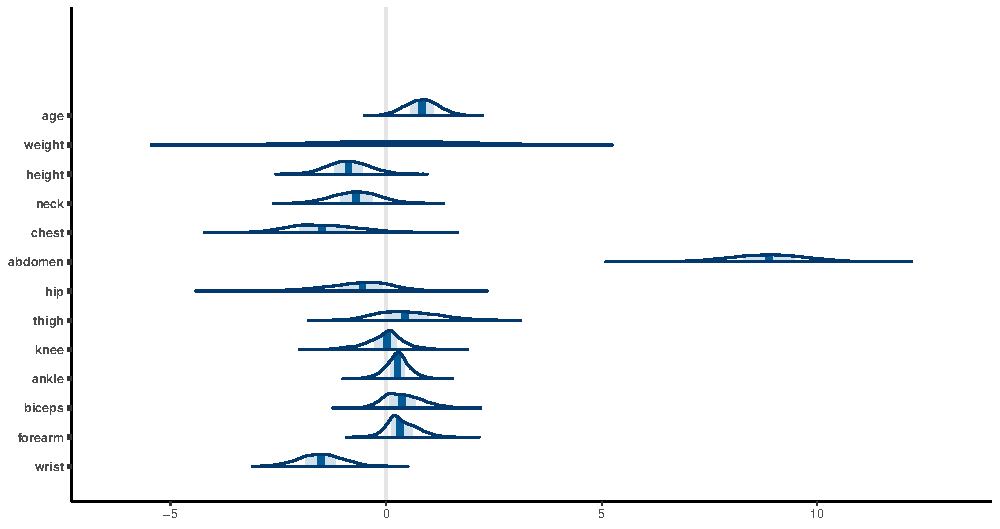
\includegraphics[width=11cm]{bodyfat_mcmc_areas_small.pdf}

\end{frame}

\begin{frame}
  
  {\Large\color{navyblue} Bodyfat}

  Marginal posteriors of coefficients ({\color{red} Much better!})
  
  \includegraphics[width=11cm]{bodyfat_mcmc_areas.pdf}

\end{frame}

\begin{frame}[fragile]
  
  {\Large\color{navyblue} Figure font size}

For example:
  
  {\footnotesize
\begin{lstlisting}
theme_set(bayesplot::theme_default(base_family = "sans",
          base_size=16))
\end{lstlisting}
  }

\end{frame}


\begin{frame}
  
  {\Large\color{navyblue} Bodyfat}

  Bivariate marginal of weight and height
  
  \includegraphics[width=7.5cm]{bodyfat_mcmc_scatter.pdf}

\end{frame}

\begin{frame}
  
  {\Large\color{navyblue} Bodyfat variable selection}

  \begin{itemize}
  \item<1-> Do we need all the measurements?
  \item<1-> We find the model with a minimal set of variables which have similar predictive performance as the model with all variables
  \item<2-> We use projection predictive variable selection
    implemented in {\tt projpred} package
\end{itemize}
\end{frame}

\begin{frame}

  {\Large\color{navyblue} {Projective predictive covariate selection}}
    
\begin{itemize}
\item The full model predictive distribution represents our best knowledge about future $\tilde{y}$
	\begin{align*}
          p(\tilde{y} | D) = \int p(\tilde{y} | \vs\theta) p(\vs \theta| D) d\vs\theta,
        \end{align*}
        where $\vs \theta=(\vs \beta,\sigma^2)$) and $\vs \beta$ is in general non-sparse (all $\vs\beta_j \ne 0$)
	% \item The predictive distribution $p(\tilde{y} \given D) \sim \frac{1}{S}\sum_s p(\tilde{y} \given \vs \theta^s)$ 
	\item What is the best distribution $q_\perp(\vs \theta)$ given a
          constraint that only selected covariates have nonzero coefficient
          % ($||\vs \beta||_0 = k)$?
	\item Optimization problem:
	\begin{align*}
		q_\perp = \arg \min_{q} \frac{1}{n} \sum_{i=1}^n 
			\KLx{p(\tilde{y}_i \mid D)}{\int p(\tilde{y}_i \mid \vs \theta) q(\vs \theta) d\vs\theta}%,\\ \subjto\, ||\vs \beta||_0 = k
	\end{align*}
      \item Optimal projection from the full posterior to a sparse
        posterior (with minimal predictive loss)
\end{itemize}

\end{frame}

\begin{frame}

  {\Large\color{red} {For 10min presentation, too much information}}


\begin{itemize}
    \color{gray}
\item The full model predictive distribution represents our best knowledge about future $\tilde{y}$
	\begin{align*}
          p(\tilde{y} | D) = \int p(\tilde{y} | \vs\theta) p(\vs \theta| D) d\vs\theta,
        \end{align*}
        where $\vs \theta=(\vs \beta,\sigma^2)$) and $\vs \beta$ is in general non-sparse (all $\vs\beta_j \ne 0$)
	% \item The predictive distribution $p(\tilde{y} \given D) \sim \frac{1}{S}\sum_s p(\tilde{y} \given \vs \theta^s)$ 
	\item What is the best distribution $q_\perp(\vs \theta)$ given a
          constraint that only selected covariates have nonzero coefficient
          % ($||\vs \beta||_0 = k)$?
	\item Optimization problem:
	\begin{align*}
		q_\perp = \arg \min_{q} \frac{1}{n} \sum_{i=1}^n 
			\KLx{p(\tilde{y}_i \mid D)}{\int p(\tilde{y}_i \mid \vs \theta) q(\vs \theta) d\vs\theta}%,\\ \subjto\, ||\vs \beta||_0 = k
	\end{align*}
      \item Optimal projection from the full posterior to a sparse
        posterior (with minimal predictive loss)
\end{itemize}


\end{frame}


\begin{frame}
  
  {\Large\color{navyblue} Bodyfat}

  \only<1>{The predictive performance of the full and submodels

      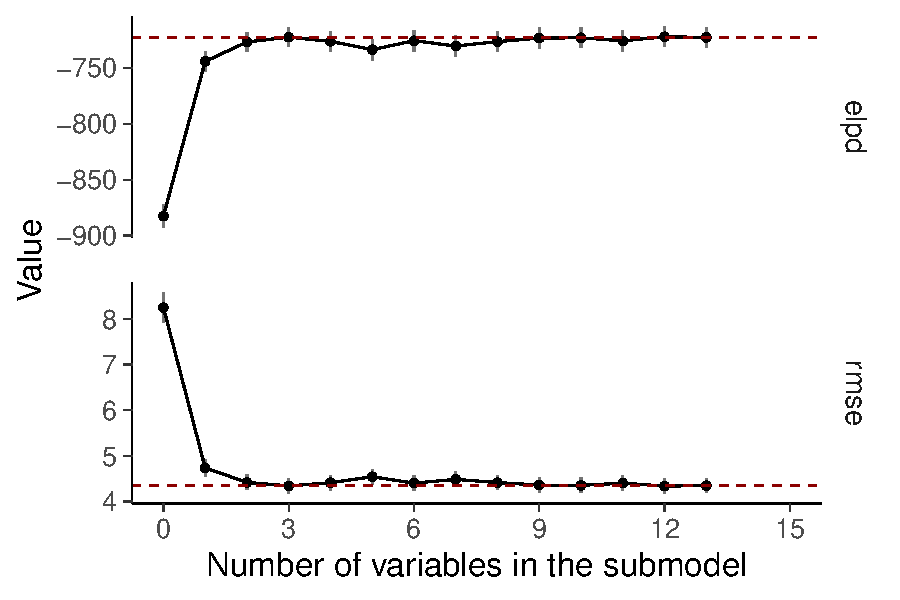
\includegraphics[width=11cm]{bodyfat_varsel_plot2.pdf}
  }
  \only<2>{The predictive performance of the full and submodels

    {\color{gray} One of these plots is probably sufficient}
    
      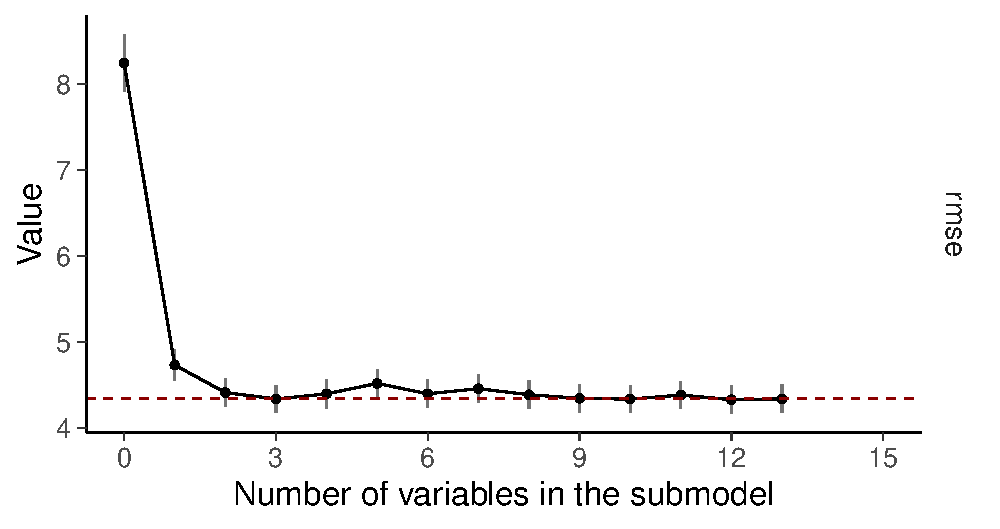
\includegraphics[width=11cm]{bodyfat_varsel_plot_rmse.pdf}
    }
  

\end{frame}


\begin{frame}
  
  {\Large\color{navyblue} Bodyfat}

  Marginals of projected posterior
  
  \includegraphics[width=11cm]{bodyfat_proj_mcmc_areas.pdf}

\end{frame}

% \begin{frame}
  
%   {\Large\color{navyblue} Bodyfat}

%   Projected posterior is not just the conditional of joint
  
%   \includegraphics[width=7.5cm]{bodyfat_proj_mcmc_scatter.pdf}

% \end{frame}


% \begin{frame}
  
%   {\Large\color{navyblue} Bodyfat}

%   Projected posterior is different than posterior conditioned only on selected features

%   \vspace{-0.7\baselineskip}
%   \includegraphics[width=11cm]{bodyfat_compare_sigmas.pdf}

% \end{frame}

% Case study \url{avehtari.github.io/modelselection/bodyfat.html}
% \begin{frame}
  
%   {\Large\color{navyblue} Projection of Gaussian graphical models}\\

%   \begin{itemize}
%   \item Williams, Piironen, Vehtari, Rast (2018). Bayesian estimation of Gaussian graphical models with projection predictive selection. \href{https://arxiv.org/abs/1801.05725}{arXiv:1801.05725}\\
%     \includegraphics[width=8.5cm]{ceu.pdf}\\
%     {\footnotesize CEU genetic network. BGL: Bayesian glasso; GL: glasso;
%       TIGER: tuning insensitive graph estimation and regression; BMA:
%       Bayesian model averaging; MAP: Maximum a posteriori; Projection:
%       projection predictive selection.}
%   \end{itemize}
  
% \end{frame}

% \begin{frame}
  
%   {\Large\color{navyblue} More results}\\

%   {\footnotesize
%   \begin{itemize}
%   \item More results projpred vs. Lasso and elastic net:\\
%     Piironen, Paasiniemi, Vehtari (2018). Projective Inference in
%     High-dimensional Problems: Prediction and Feature Selection.
%     \href{https://arxiv.org/abs/arXiv:1810.02406}{arXiv:1810.02406}
%   \item More results projpred vs. marginal posterior probabilities:\\
%     Piironen and Vehtari (2017). Comparison of Bayesian predictive
%     methods for model selection. Statistics and Computing,
%     27(3):711-735.
%     \href{https://dx.doi.org/10.1007/s11222-016-9649-y}{doi:10.1007/s11222-016-9649-y}.
%   \item projpred for Gaussian graphical models:\\
%     Williams, Piironen, Vehtari, Rast (2018). Bayesian estimation of Gaussian graphical models with projection predictive selection. \href{https://arxiv.org/abs/1801.05725}{arXiv:1801.05725}
%   \item More results for Bayes SPC:\\
%     Piironen and Vehtari (2018). Iterative supervised principal components. 21st AISTATS, PMLR 84:106-114. \href{http://proceedings.mlr.press/v84/piironen18a.html}{Online}.
%   \item Several case studies for small to moderate dimensional ($p=4 \ldots 100$) small data:\\
%     Vehtari (2018). Model assesment, selection and inference after
%     selection. \url{https://avehtari.github.io/modelselection/}
%   \end{itemize}
%   }
% \end{frame}


\frame{

  {\Large\color{navyblue} Bodyfat -- Conclusion}

\begin{itemize}
\item<1-> Bodyfat percentage estimated using water immersion can be
  predicted using scale and tape measure
\item<2-> The accuracy using mean of data is 16\%-units (95\% interval)
\item<3-> The accuracy using all anthropometric measures is 8.6\%-units
  (95\% interval)
\item<4-> The same accuracy can be obtained using just abdomen
  circumference and weight
\item<5-> More results at \url{avehtari.github.io/modelselection/bodyfat.html}
\end{itemize}
}

{\setbeamertemplate{footline}[]
  \author[]{Aki Vehtari}
  \begin{frame}{}

  \centering

  \vspace{4\baselineskip}

  \only<1>{\huge\color{navyblue}  THANKS!}
  \only<2->{{\color{red} \huge NO ``THANKS''!}}

  \vspace{2\baselineskip}

    \begin{itemize}
    \item<3-> Don't ever end with a slide having just ``THANKS''
    \item<4-> ``THANKS'' slide has zero information content
    \item<5-> Leave the conclusion slide or contact information slide
    \end{itemize}
  
\end{frame}
}

\frame{

  {\Large\color{navyblue} Conclusion}

\begin{itemize}
\item Bodyfat percentage estimated using water immersion can be
  predicted using scale and tape measure
\item The accuracy using mean of data is 16\%-units (95\% interval)
\item The accuracy using all anthropometric measures is 8.6\%-units
  (95\% interval)
\item The same accuracy can be obtained using just abdomen
  circumference and weight
\item More results at \url{avehtari.github.io/modelselection/bodyfat.html}
\end{itemize}
}

\begin{frame}[fragile]

  {\Large\color{navyblue} Additional information}

  \begin{itemize}
  \item You can have additional slides after the conclusion for
    supporting material to answer questions
    \begin{itemize}
    \item for example, in this course, include Stan code and
      additional convergence and model checking results
    \end{itemize}
  \end{itemize}

Gaussian linear model with regularized horseshoe prior
  
  {\tiny
\begin{lstlisting}
// generated with brms 2.14.4
functions {
  vector horseshoe(vector z, vector lambda, real tau, real c2) {
    int K = rows(z);
    vector[K] lambda2 = square(lambda);
    vector[K] lambda_tilde = sqrt(c2 * lambda2 ./ (c2 + tau^2 * lambda2));
    return z .* lambda_tilde * tau;
  }
}
data {
  int<lower=1> N;  // total number of observations
  vector[N] Y;  // response variable
  int<lower=1> K;  // number of population-level effects
  matrix[N, K] X;  // population-level design matrix
  // data for the horseshoe prior
  real<lower=0> hs_df;  // local degrees of freedom
  real<lower=0> hs_df_global;  // global degrees of freedom
  real<lower=0> hs_df_slab;  // slab degrees of freedom
  real<lower=0> hs_scale_global;  // global prior scale
  real<lower=0> hs_scale_slab;  // slab prior scale
  int prior_only;  // should the likelihood be ignored?
}
transformed data {
  int Kc = K - 1;
  matrix[N, Kc] Xc;  // centered version of X without an intercept
  vector[Kc] means_X;  // column means of X before centering
  for (i in 2:K) {
    means_X[i - 1] = mean(X[, i]);
    Xc[, i - 1] = X[, i] - means_X[i - 1];
  }
}
parameters {
  // local parameters for horseshoe prior
  vector[Kc] zb;
  vector<lower=0>[Kc] hs_local;
  real Intercept;  // temporary intercept for centered predictors
  // horseshoe shrinkage parameters
  real<lower=0> hs_global;  // global shrinkage parameters
  real<lower=0> hs_slab;  // slab regularization parameter
  real<lower=0> sigma;  // residual SD
}
transformed parameters {
  vector[Kc] b;  // population-level effects
  // compute actual regression coefficients
  b = horseshoe(zb, hs_local, hs_global, hs_scale_slab^2 * hs_slab);
}
model {
  // likelihood including all constants
  if (!prior_only) {
    target += normal_id_glm_lpdf(Y | Xc, Intercept, b, sigma);
  }
  // priors including all constants
  target += std_normal_lpdf(zb);
  target += student_t_lpdf(hs_local | hs_df, 0, 1)
    - rows(hs_local) * log(0.5);
  target += student_t_lpdf(Intercept | 3, 19.2, 9.2);
  target += student_t_lpdf(hs_global | hs_df_global, 0, hs_scale_global * sigma)
    - 1 * log(0.5);
  target += inv_gamma_lpdf(hs_slab | 0.5 * hs_df_slab, 0.5 * hs_df_slab);
  target += student_t_lpdf(sigma | 3, 0, 9.2)
    - 1 * student_t_lccdf(0 | 3, 0, 9.2);
}
generated quantities {
  // actual population-level intercept
  real b_Intercept = Intercept - dot_product(means_X, b);
}
\end{lstlisting}
  }


\end{frame}

\begin{frame}{}

  {\Large\color{navyblue} Classification example: Pima Indians Diabetes}

  Predict diabetes based on
  \begin{itemize}
  \item Pregnancies
  \item Glucose
  \item Blood pressure
  \item Skin thickness
  \item Insulin
  \item BMI
  \item Diabetes Pedigree
  \item Age
  \end{itemize}

  768 observations

  \vspace{2\baselineskip}

  \url{https://avehtari.github.io/modelselection/diabetes.html}
  
\end{frame}

\begin{frame}{}

  {\Large\color{navyblue} Classification example: Pima Indians Diabetes}

  Leave-one-out cross-validation classification accuracy 78\%

  \uncover<2->{
  Calibration:\\
    \includegraphics[width=10.5cm]{binary_model_calibration.pdf}

    }
  
\end{frame}

\begin{frame}{}

  {\Large\color{navyblue} Hierarchical example: Rats growth curves}

  \includegraphics[width=10.5cm]{rats_data.pdf}

  \url{https://avehtari.github.io/modelselection/rats_kcv.html}
  
\end{frame}

\begin{frame}[fragile]

  {\Large\color{navyblue} Hierarchical example: Rats growth curves}

Simple linear model
{\footnotesize
\begin{lstlisting}
fit_1 <- stan_glm(weight ~ age, data=dfrats)
\end{lstlisting}
}

Linear model with hierarchical intercept
{\footnotesize
\begin{lstlisting}
fit_2 <- stan_glmer(weight ~ age + (1 | rat), data=dfrats)
\end{lstlisting}
}

 Linear model with hierarchical intercept and slope
{\footnotesize
\begin{lstlisting}
fit_3 <- stan_glmer(weight ~ age + (age | rat), data=dfrats)
\end{lstlisting}
}

 \uncover<2->{
Instead of \texttt{stan\_glm(er)}, use \texttt{brm} to get the Stan code, too.
}
\end{frame}

\begin{frame}[fragile]

  {\Large\color{navyblue} Hierarchical example: Rats growth curves}

Leave-one-out cross-validation
{\footnotesize
\begin{lstlisting}
                                 elpd_diff se_diff
hierarchical intercept and slope    0.0       0.0 
hierarchical intercept            -23.6       9.3 
simple linear model              -109.6      13.3 
\end{lstlisting}
}


\end{frame}

\begin{frame}[fragile]

  {\Large\color{navyblue} Hierarchical example: Rats growth curves}

Leave-one-out cross-validation
{\footnotesize
\begin{lstlisting}
                                 elpd_diff se_diff
hierarchical intercept and slope    0.0       0.0 
hierarchical intercept            -23.6       9.3 
simple linear model              -109.6      13.3 
\end{lstlisting}
}

Leave-one-out cross-validation stacking model weights
{\footnotesize
\begin{lstlisting}
                                  weight
hierarchical intercept and slope   0.93
hierarchical intercept             0.07 
simple linear model                0.00
\end{lstlisting}
}

\end{frame}

\end{document}

\begin{frame}

{\Large\color{navyblue} Bayesian stacking}

  \begin{itemize}
  \item Consider the model averaging as a decision problem with aim of
    maximizing the predictive performance
  \item<2-> Maximize the scoring rule of the predictive distribution for future $\tilde{y}$
    \begin{align*} \label{stacking_population}
      \max_{w}  S\Bigl(   \sum_{k=1}^K w_k p(\tilde{y} | x, y, M_k), p_t(\tilde{y}) \Bigr),  
    \end{align*}
  \item<3-> As we don't know $p_t(\tilde{y})$, we approximate with LOO
  \item<4-> We define the stacking weights as the solution to the following optimization problem:
\begin{align*} 
 \max_w \frac{1}{n}\sum_{i=1}^n S\Bigl( \sum_{k=1}^K  w_k \hat p(y_i|x_{-i},y_{-i},M_k) \Bigr) ,\\ \quad  s.t. \quad w_k \geq 0,   \quad \sum_{k=1}^K w_k=1.
\end{align*}
  \end{itemize}

\end{frame}

\begin{frame}

{\Large\color{navyblue} Bayesian stacking}

  \begin{itemize}
\item The combined estimation of the predictive density is
 \begin{align*} 
  \hat p(\tilde{y} |x, y)= \sum_{k=1}^K \hat{w}_k p(\tilde{y}|x, y, M_k).
  \end{align*}
\item<2-> When using log-score (corresponding to Kullback-Leibler
  divergence), we call this \emph{stacking of predictive
    distributions}:
\begin{align*}
  \max_w \frac{1}{n} \sum_{i=1}^n \log \sum_{k=1}^K w_k p(y_i | x_{-i}, y_{-i}, M_k) , \\
  \quad s.t.   \quad w_k \geq 0,   \quad \sum_{k=1}^K w_k=1.
\end{align*}
  \item<3-> We can approximate $p(y_i | x_{-i}, y_{-i}, M_k)$ with PSIS-LOO
  \item<4-> Other cross-validation structures can be used, too
  \end{itemize}
\end{frame}

\begin{frame}

{\Large\color{navyblue} Gaussian mixture example}

$y \sim \N(3.4, 1), \quad p_k = \N(k, 1) \text{ with } k = 1,\ldots,8$
\pause

Model averaged predictive distributions
 \includegraphics[width=12cm]{dis34.pdf}

\end{frame}

\begin{frame}

{\Large\color{navyblue} Gaussian mixture example}

$y \sim \N(3.4, 1), \quad p_k = \N(k, 1) \text{ with } k = 1,\ldots,8$

(a, b) {\color{red} Stacking of predictive distributions} vs. {\color{greenish} BMA}\\
  \vspace{0.2cm}

   \makebox[12cm][t]{
  \hspace{-0.7cm}
\begin{overlayarea}{12cm}{4.5cm}
 \includegraphics[width=12cm]{score34.pdf}\\
 \only<1>{\hide[white]{-0.4}{0.65}{0.4}{0.33}} %
\end{overlayarea}
}

\uncover<2->{
(c) Dilutation of prior by adding copies of $\N(4,1)$ to the model space
}

\end{frame}

\begin{frame}

{\Large\color{navyblue} Linear subset regression example $k$}

\vspace{-0.4\baselineskip}
$y \sim \N(\mu, 1), \quad \mu = \beta_1 X_1 + \ldots \beta_{15} X_{15}$\\
\only<1>{\makebox[12cm][t]{\scriptsize
$ \beta_j=\gamma\left(     (1_{ | j-4 | <h}  (h- |j-4|)^2  +(  1_{|j-8|<h }   )  (  h- |j-8|  )^2+ (   1_{|j-12|<h}    ) (  h-|j-12|  )^2 \right)$
}}

\pause
Non-nested $M$-open case with $M_k: \N(\beta_k X_k, \sigma)$\\ \pause
\vspace{-\baselineskip}
\makebox[12cm][t]{
  \hspace{-0.7cm}
\includegraphics[width=10.4cm]{single_variable_regression.pdf}
}\\
\vspace{-0.5\baselineskip}
(a) {\color{red}Stacking}, (b) {\color{red}BMA},
(d) model selection by {\color{red}LOO} and {\color{blue}BF}\\
{\vspace{-5.5cm}\hspace{2.4cm}(a)}{\hspace{4.2cm}(b)}\\
{\vspace{2.5cm}\hspace{7.1cm}(d)}

\end{frame}

\begin{frame}

{\Large\color{navyblue} Linear subset regression example $1:k$}

\vspace{-0.4\baselineskip}
$y \sim \N(\mu, 1), \quad \mu = \beta_1 X_1 + \ldots \beta_{15} X_{15}$\\
Nested $M$-closed case with $M_k: \N( \sum_{j=1}^k \beta_j X_j, \sigma)$\\ \pause
\vspace{-\baselineskip}
\makebox[12cm][t]{
  \hspace{-0.7cm}
  \includegraphics[width=10.4cm]{linear_regression.pdf}
}\\
\vspace{-0.5\baselineskip}
(a) {\color{red}Stacking}, (b) {\color{red}BMA},
(d) model selection by {\color{red}LOO} and {\color{blue}BF}\\
{\vspace{-5.5cm}\hspace{2.4cm}(a)}{\hspace{4.2cm}(b)}\\
{\vspace{2.5cm}\hspace{7.1cm}(d)}


\end{frame}

\begin{frame}

{\Large\color{navyblue} Variational multimodal example}

Stacking of predictive distributions can be helpful also in case of
multimodal posteriors\\
\vspace{-\baselineskip}
\makebox[12cm][t]{
  \hspace{-0.7cm}
  \includegraphics[width=12.5cm]{vb.pdf}
}

\end{frame}

%\begin{frame}

% {\Large\color{navyblue} Non-linear model example}

%   \begin{center}
%   \includegraphics[width=\textwidth]{wells.pdf}
%   \end{center}

% \end{frame}

% \begin{frame}

% {\Large\color{navyblue} Non-linear model example}

%   \begin{center}
%   \includegraphics[width=\textwidth]{wells_combine.pdf}
%   \end{center}

% \end{frame}

\begin{frame}

{\Large\color{navyblue} Bayesian stacking}
  
  \begin{itemize}
  \item In $M$-open case works better than BMA
  \item In $M$-closed case can have a better small sample performance than BMA
  \item<2-> Should be used only for model averaging
    \begin{list2}
    \item you may drop models with 0 weights
    \item you shouldn't choose the model with largest weight unless it's 1
    \end{list2}
  \item<2-> \href{https://projecteuclid.org/euclid.ba/1516093227}{Yao, Vehtari, Simpson, \& Gelman (2018)}
  \end{itemize}
  
\end{frame}


\begin{frame}{}

  {\Large\color{navyblue} Part 2: Projective Inference in
    High-dimensional Problems: Prediction and Feature
    Selection}

\end{frame}

\begin{frame}{}

  {\Large\color{navyblue} High dimensional small data}

  \begin{itemize}
  \item In the examples $n = 54...102$, $p=1536...22283$
    \begin{itemize}
    \item could scale to bigger $n$ and bigger $p$
    \end{itemize}
  \item<2-> Priors necessary
    \begin{itemize}
    \item shrinkage priors, hierarchical shrinkage priors
    \item dimension reduction with factor models
    \end{itemize}
    \vspace{\baselineskip}
  \item<3-> The main content of this part: Two stage approach
    \begin{itemize}
    \item Construct a best predictive model you can\\ $\Rightarrow$ {\it reference model}
    \item Feature selection and post-selection inference\\ $\Rightarrow$ {\it projection}
    \end{itemize}
  \end{itemize}
  
\end{frame}

\begin{frame}{}

  {\Large\color{navyblue} Rich model vs feature selection?}

  \begin{itemize}
  \item If we care only about the predictive performance
    \begin{itemize}
    \item Include all available prior information
    \item Integrate over all uncertainties
    \item No need for feature selection
    \end{itemize}
  \item<2-> Variable selection can be useful if
    \begin{itemize}
    \item need to reduce measurement or computation cost in the future
    \item improve explainability
    \end{itemize}
  \item<3-> Two options for variable selection
    \begin{itemize}
    \item Find a minimal subset of features that yield a good
      predictive model
    \item Identify all features that have predictive information
    \end{itemize}
  \end{itemize}
  
\end{frame}

\begin{frame}{}

  {\Large\color{navyblue} Regularized horseshoe prior}
  
  \vspace{-0.3\baselineskip}
  \begin{itemize}
  \item Horseshoe: can be seen as continuos version of spike-and-slab with
    {\it infinite} width slab
    \begin{itemize}
    \item no shrinkage ($\kappa_j \rightarrow 0$) allows complete separation in logistic model with $n \ll p$\\
      \vspace{0.5\baselineskip}
      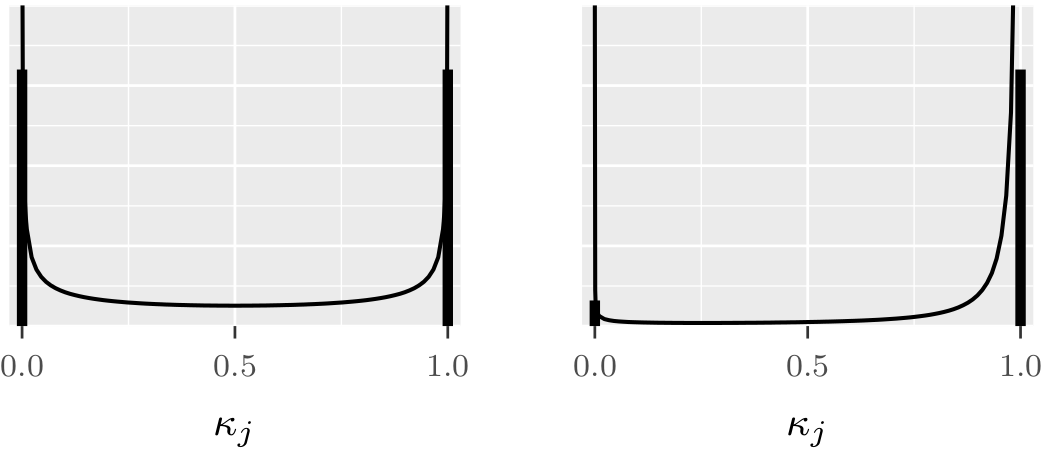
\includegraphics[width=5.5cm]{hs_vs_spikeandslab.png}
    \end{itemize}
    % \vspace{0.5\baselineskip}
  \item<2-> Regularized horseshoe: adds additional {\it finite} width slab
    \begin{itemize}
    \item some minimal shrinkage ($\kappa_j > 0$) for relevant features, but maintains division to relevant and non-relevant features\\
      \vspace{0.5\baselineskip}
      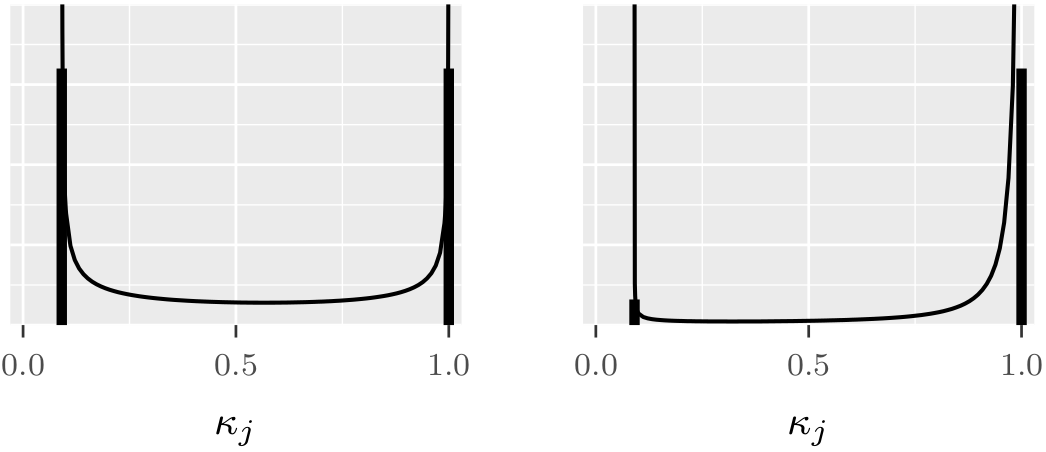
\includegraphics[width=5.5cm]{rhs_vs_spikeandslab.png}
    \end{itemize}
  \end{itemize}
\end{frame}

\begin{frame}

  {\Large\color{navyblue} Regularized horseshoe}

  \begin{itemize}
    \item {\small Piironen and Vehtari (2017). Sparsity information and
      regularization in the horseshoe and other shrinkage priors. In
      Electronic Journal of Statistics, 11(2):5018-5051. \href{https://projecteuclid.org/euclid.ejs/1513306866}{Online}}
      \begin{itemize}
      \item regularized horseshoe
      \item how to set the prior based on the sparsity assumption
      \end{itemize}
  \end{itemize}

\end{frame}

\begin{frame}{}

  {\Large\color{navyblue} Why shrinkage priors alone do not solve the
    variable selection problem}

  \begin{itemize}
  \item A common strategy:
    \begin{itemize}
    \item Fit model with a shrinkage prior
    \item Select variables based on marginal posteriors (of the
      regression coefficients)
    \end{itemize}
  \item<2-> Problems
    \begin{itemize}
    \item Marginal posteriors are difficult with correlated features
    \item How to do post-selection inference correctly?
    \end{itemize}
  \end{itemize}
\end{frame}

\begin{frame}{}

  {\Large\color{navyblue} Example}

Consider data
\begin{equation*}
  \color{gray}
\begin{alignedat}{2}
  \only<1>{\color{black}}f & \only<1>{\color{black}} \sim \N(0,1), &&  \\
  \only<2>{\color{black}}y \mid f &\only<2>{\color{black}}\sim \N(f, 1) && \\
  \only<3>{\color{black}}x_j \mid f &\only<3>{\color{black}}\sim \N(\sqrt{\rho}f,\, 1-\rho), \qquad &&\only<3>{\color{black}} j = 1,\dots,25 \,, \\
  \only<4>{\color{black}}x_j \mid f &\only<4>{\color{black}}\sim \N(0, 1), && \only<4>{\color{black}}j = 26,\dots, 50 \,.
\end{alignedat}
\end{equation*}

\begin{itemize}
\item<2-> $y$ are noisy observations about latent $f$ \pause
\item<3-> First $p_\text{rel}=25$ features are correlated with $\rho$ and predictive about $y$ \pause
\item<4-> Remaining $25$ features are irrelevant random noise
\end{itemize}
\uncover<5>{Generate one data set $\{ x^{(i)}, y^{(i)}\}^n_{i=1}$ with $n=50$ and $\rho=0.8$ and assess the feature relevances}

\end{frame}

\begin{frame}{}

  {\Large\color{navyblue} Example}

  \makebox[12.1cm][t]{
    \hspace{-0.9cm}
  \begin{minipage}[b][4cm][t]{12.1cm}
  \includegraphics[width=4cm]{toy_marginal1.pdf}
  \uncover<2->{\includegraphics[width=4cm]{toy_marginal2.pdf}}
  \uncover<3->{\includegraphics[width=4cm]{toy_marginal3.pdf}}\\
\end{minipage}
}\\
\uncover<1->{
	A) Gaussian prior, posterior median with 50\% and 90\% intervals\\ 
	}
	\uncover<2->{
	B) Horseshoe prior, same things\\ 
	}
	\uncover<3->{
	C) Spike-and-slab prior, posterior inclusion probabilities\\ 
      }
      ~\\
      \uncover<4>{Half of the features relevant, but all marginals
        substantially overlapping with zero}
\end{frame}

\begin{frame}{}

  {\Large\color{navyblue} What happens?}

  \makebox[12.1cm][t]{
    \hspace{-0.3cm}
    \begin{minipage}[b][8.1cm][t]{12.1cm}
      \makebox[0cm][t]{\hspace{-0.4cm}\rotatebox{90}{\hspace{1.4cm}Gaussian}}
      \includegraphics[width=3.7cm]{toy_scatter1.pdf}
      \uncover<2->{\includegraphics[width=3.7cm]{toy_scatter3.pdf}}
      \uncover<3->{\includegraphics[width=3.7cm]{toy_scatter5.pdf}}\\
      \makebox[0cm][t]{\hspace{-0.4cm}\rotatebox{90}{\hspace{1.4cm}Horseshoe}}
      \includegraphics[width=3.7cm]{toy_scatter2.pdf}
      \uncover<2->{\includegraphics[width=3.7cm]{toy_scatter4.pdf}}
      \uncover<3->{\includegraphics[width=3.7cm]{toy_scatter6.pdf}}\\
      \makebox[3.7cm]{$\quad p_\text{rel}=2$}
      \uncover<2->{\makebox[3.7cm]{$\quad p_\text{rel}=5$}}
      \uncover<3->{\makebox[3.7cm]{$\quad p_\text{rel}=25$}}
\end{minipage}
}
\end{frame}

\begin{frame}{}

  {\Large\color{navyblue} Focus on predictive performance}

  \begin{itemize}
  \item Two stage approach
    \begin{itemize}
    \item Construct a best predictive model you can\\ $\Rightarrow$ {\it reference model}
    \item Variable selection and post-selection inference\\ $\Rightarrow$ {\it projection}
    \end{itemize}
  \item<2-> Instead of looking at the marginals, find the minimal
    subset of features which have (almost) the same predictive
    performance as the reference model
  \end{itemize}
  
\end{frame}

\begin{frame}{}

  {\Large\color{navyblue} Reference model improves variable selection}

  Same data generating mechanism, but\\ $n=30$, $p=500$, $p_\text{rel}=150$, $\rho=0.5$.

  \includegraphics[width=5.5cm]{toy_corr1.pdf}\\
  \vspace{-0.2cm}
  \hspace{0.5cm} {\color{set12} irrelevant $x_j$}, {\color{set11} relevant $x_j$}\\
  \vspace{0.2cm}
  \hspace{0.5cm} Sample correlation with $y$\\
  
\end{frame}

\begin{frame}{}

  {\Large\color{navyblue} Reference model improves variable selection}

  \includegraphics[width=5.5cm]{toy_corr2.pdf}
  \uncover<2->{\includegraphics[width=5.5cm]{toy_corr3.pdf}}\\
  \vspace{-0.2cm}
  \hspace{0.5cm} {\color{set12} irrelevant $x_j$}, {\color{set11} relevant $x_j$}\\
  \vspace{0.2cm}
  A) Sample correlation with $y$ vs. sample correlation with $f$\\
  \uncover<2->{B) Sample correlation with $y$ vs. sample correlation with $f_*$\\
  $f_* = $ linear regression fit with 3 supervised principal components}
  
\end{frame}

\begin{frame}{}

  {\Large\color{navyblue} (Iterative) Supervised Principal Components}

  \begin{itemize}
  \item Dimension reduction for high dimensional small data with
    highly correlating features
    \begin{itemize}
    \item dimension reduction helps to speed up later computation
      without discarding much information
    \item supervised means that features correlating with the target
      are favored in construcing the principal components
    \end{itemize}
    {\small
    \item     Piironen and Vehtari (2018). Iterative supervised principal components. 21st AISTATS, PMLR 84:106-114. \href{http://proceedings.mlr.press/v84/piironen18a.html}{Online}.
    }
  \end{itemize}
  
\end{frame}

\begin{frame}{}

  {\Large\color{navyblue} Predictive projection, idea}
  
  \begin{itemize}
  \item Model simplification technique
  \item<2-> Replace full posterior $p(\theta \mid D)$ with
    some constrained $q(\theta)$ so that the \emph{predictive
      distribution} changes as little as possible
  \item<3-> Example constraints
    \begin{itemize}
    \item $q(\theta)$ can have only point mass at some $\theta_0$ \\
      $\Rightarrow$ ``Optimal point estimates''
    \item<4-> Some features must have exactly zero regression coefficient \\
      $\Rightarrow$ ``Which features can be discarded''
    \end{itemize}
    \vspace{1\baselineskip}
  \item<5-> The decision theoretic idea of conditioning the smaller
    model inference on the full model can be tracked to Lindley (1968)
    \begin{itemize}
    \item draw by draw projection introduced by Goutis \& Robert
      (1998), and Dupuis \& Robert (2003)
    \item see also many related references in a review by
      \href{http://dx.doi.org/10.1214/12-SS102}{Vehtari \& Ojanen
        (2012)}
    \end{itemize}
\end{itemize}

\end{frame}

\begin{frame}{}

  {\Large\color{navyblue} Logistic regression with two features}

  \vspace{\baselineskip}
  
  \begin{overlayarea}{\textwidth}{0.7\textwidth}
    \begin{minipage}{0.99\textwidth}
      \begin{center}
        \only<1>{ \minput{proj_posterior} }%
        \only<2>{ \minput{proj_b1b2_single} }%
        \only<3>{ \minput{proj_b2_single} }%
        \only<4>{ \minput{proj_b1_single} }%
        \only<5>{ \minput{proj_b2_dbd} }%
        \only<6>{ \minput{proj_b1_dbd} }%
      \end{center}
    \end{minipage}
    \begin{minipage}{0.99\textwidth}
      \only<1>{Full posterior for $\beta_1$ and $\beta_2$ and contours of predicted class probability}
      \only<2>{Projected point estimates for $\beta_1$ and $\beta_2$}
      \only<3>{Projected point estimates, constraint $\beta_1 = 0$}
      \only<4>{Projected point estimates, constraint $\beta_2 = 0$}
      \only<5>{Draw-by-draw projection, constraint $\beta_1 = 0$}
      \only<6>{Draw-by-draw projection, constraint $\beta_2 = 0$}
    \end{minipage}
  \end{overlayarea}
\end{frame}

\begin{frame}

  {\Large\color{navyblue} Predictive projection}


  \begin{itemize}
  \item Replace full posterior $p(\theta \mid D)$ with some
    constrained $q(\theta)$ so that the \emph{predictive distribution}
    changes as little as possible
  \item<2-> As the full posterior $p(\theta \mid D)$ is projected to $q(\theta)$
    \begin{itemize}
    \item the prior is also projected and there is no need to define
      priors for submodels separately
    \item<3-> even if we constrain some coefficients to be $0$, the
      predictive inference is conditoned on the information related
      features contributed to the reference model
    \end{itemize}
  \end{itemize}

  
\end{frame}

\frame{

  {\Large\color{navyblue} Projective selection}

\begin{itemize}
	\item How to select a feature combination? \pause
	\item For a given model size, choose feature combination with minimal projective loss \pause
	\item Search heuristics, e.g. 
	\begin{itemize}
        \item Monte Carlo search
        \item Forward search
        \item $L_1$-penalization (as in Lasso)
	\end{itemize} \pause 
      \item Use cross-validation to select the appropriate model size
        \begin{itemize}
        \item need to cross-validate over the search paths
        \end{itemize}
      \end{itemize} 
}

\frame{

  {\Large\color{navyblue} Projective selection vs. Lasso}

Same simulated regression data as before, \\
$n=50$, $p=500$, $p_\text{rel} = 150$, $\rho=0.5$

\vspace{0.5em}

  \makebox[12.1cm][t]{
    \hspace{-0.5cm}
  \begin{minipage}{0.99\textwidth}
      \only<1>{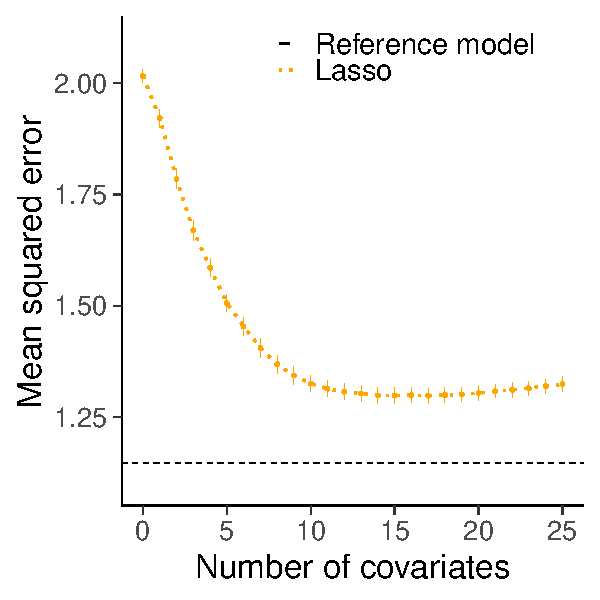
\includegraphics[width=5.5cm]{vslasso1rmse.pdf}}
      \only<2>{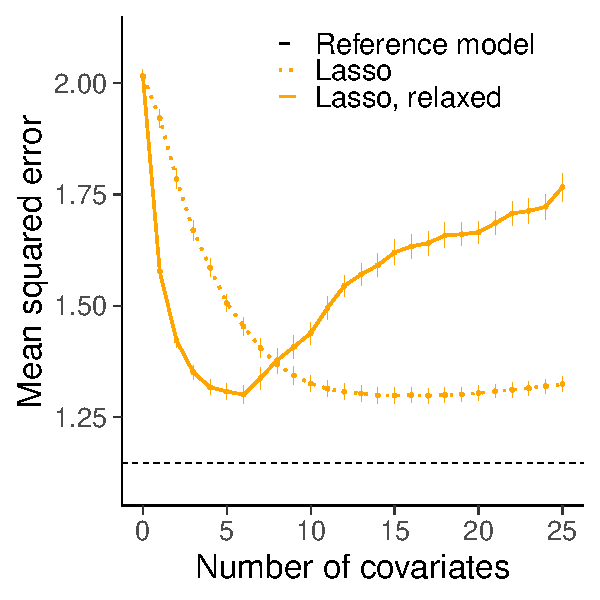
\includegraphics[width=5.5cm]{vslasso2rmse.pdf}}
      \only<3->{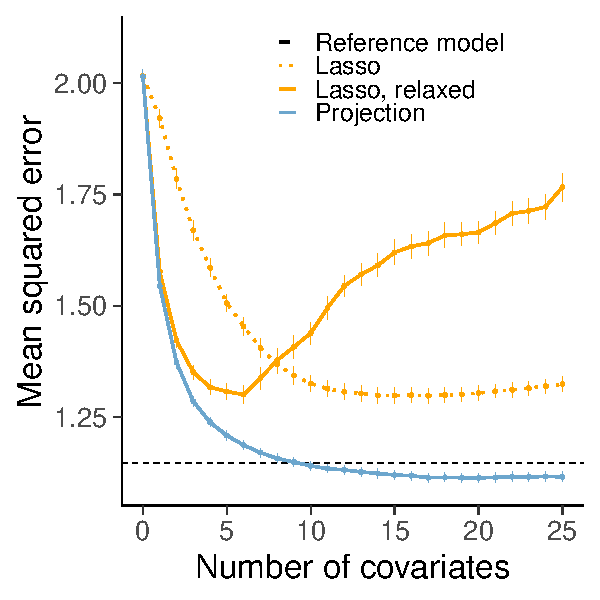
\includegraphics[width=5.5cm]{vslasso3rmse.pdf}}
      \uncover<4>{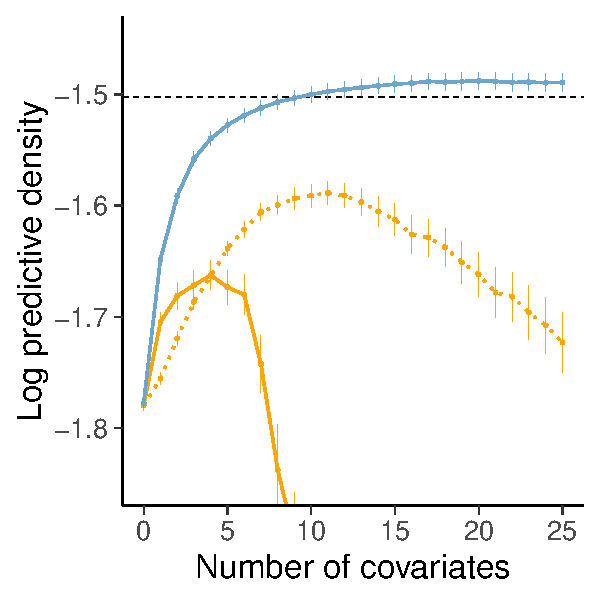
\includegraphics[width=5.5cm]{vslasso3mlpd.pdf}}
  \end{minipage}
  }
  
}

\frame{

  {\Large\color{navyblue} Real data benchmarks}\\
  $n = 54...102$, $p=1536...22283$, Bayes SPC as the reference
\begin{overlayarea}{\textwidth}{0.7\textwidth}
\vspace{-0.5em}
	\begin{minipage}{0.99\textwidth}
	\begin{center}
          \minput[pdf]{realdata}
	\end{center}
	% hidings
	\only<1>{ \hide[white]{-0.5}{-0.02}{0.42}{1.05} }%
	\only<2>{ \hide[white]{-0.3}{-0.02}{0.22}{1.05} }%
	\only<3>{ \hide[white]{-0.07}{-0.02}{0.01}{1.05} }%
	
	\end{minipage}
	%\begin{minipage}{0.99\textwidth}
	%\end{minipage}
	
\end{overlayarea}
}

\frame{

  {\Large\color{navyblue} Computation time}

  \begin{table}%
    \small
\vspace{-0.2cm}
\centering
\abovetopsep=2pt
\begin{tabular}{ lccrrrr }
\toprule
Data set & $n$ & $p$ & \multicolumn{4}{c}{Computation time} \\
\cmidrule(r){4-7}
 & & & Bayes SPC & Projection & Lasso1 & Lasso2 \\ 
\midrule
Ovarian & 54 & 1536 & 30.4 & 3.6 & 1.3 & 0.2  \\
Colon & 62 & 2000 & 31.0 & 4.0 & 1.6 & 0.3  \\
Prostate & 102 & 5966 & 49.4 & 7.6 & 5.0 & 0.8 \\
Leukemia & 72 & 7129 & 47.0 & 6.3 & 5.6 & 0.7  \\
Glioma & 85 & 22283 & 95.8 & 14.2 & 15.6 & 2.6 \\
\bottomrule
\end{tabular}
\caption{{\it Computation times:} Average computation time (in seconds) over five repeated runs. In all cases the time contains the cross-validation of the tuning parameters and/or the model size. The first result for Lasso is computed using our software ({\tt projpred}) whereas the second result (and that of ridge) is computed using the R-package {\tt glmnet} which is more highly optimized. }
\label{tab:computation_times}
\end{table}
}

\begin{frame}

  {\Large\color{navyblue} Selection induced bias in variable selection}

  \includegraphics[height=0.88\textheight]{simulated_variability.pdf}
   \vspace{-1.5\baselineskip}
   \mbox{{\hspace{8cm} \footnotesize \href{http://link.springer.com/article/10.1007/s11222-016-9649-y}{Piironen \& Vehtari (2017)}}}

\end{frame}

\begin{frame}

  {\Large\color{navyblue} Selection induced bias in variable selection}

  \includegraphics[height=0.88\textheight]{real_searchpath.pdf}
   \vspace{-2\baselineskip}
   \mbox{{\hspace{9.5cm} \parbox[t]{12cm}{\footnotesize \href{http://link.springer.com/article/10.1007/s11222-016-9649-y}{Piironen \&\\ Vehtari (2017)}}}}

\end{frame}

\begin{frame}
  
  {\Large\color{navyblue} Bodyfat: small $p$ example of projection predictive}
  
  Predict bodyfat percentage. The reference value is obtained by
  immersing person in water. $n=251$.

  \pause
  \vspace{-0.7\baselineskip}
  \includegraphics[width=7.7cm]{bodyfat_corr.pdf}

\end{frame}

\begin{frame}
  
  {\Large\color{navyblue} Bodyfat}

  Marginal posteriors of coefficients
  
  \includegraphics[width=11cm]{bodyfat_mcmc_areas.pdf}

\end{frame}

\begin{frame}
  
  {\Large\color{navyblue} Bodyfat}

  Bivariate marginal of weight and height
  
  \includegraphics[width=7.5cm]{bodyfat_mcmc_scatter.pdf}

\end{frame}

\begin{frame}
  
  {\Large\color{navyblue} Bodyfat}

  The predictive performance of the full and submodels
  
  \includegraphics[width=11cm]{bodyfat_varsel_plot.pdf}

\end{frame}


\begin{frame}
  
  {\Large\color{navyblue} Bodyfat}

  Marginals of projected posterior
  
  \includegraphics[width=11cm]{bodyfat_proj_mcmc_areas.pdf}

\end{frame}

\begin{frame}
  
  {\Large\color{navyblue} Bodyfat}

  Projected posterior is not just the conditional of joint
  
  \includegraphics[width=7.5cm]{bodyfat_proj_mcmc_scatter.pdf}

\end{frame}


% \begin{frame}
  
%   {\Large\color{navyblue} Bodyfat}

%   Projected posterior is different than posterior conditioned only on selected features

%   \vspace{-0.7\baselineskip}
%   \includegraphics[width=11cm]{bodyfat_compare_sigmas.pdf}

% \end{frame}

% Case study \url{avehtari.github.io/modelselection/bodyfat.html}
\begin{frame}
  
  {\Large\color{navyblue} Projection of Gaussian graphical models}\\

  \begin{itemize}
  \item Williams, Piironen, Vehtari, Rast (2018). Bayesian estimation of Gaussian graphical models with projection predictive selection. \href{https://arxiv.org/abs/1801.05725}{arXiv:1801.05725}\\
    \includegraphics[width=8.5cm]{ceu.pdf}\\
    {\footnotesize CEU genetic network. BGL: Bayesian glasso; GL: glasso;
      TIGER: tuning insensitive graph estimation and regression; BMA:
      Bayesian model averaging; MAP: Maximum a posteriori; Projection:
      projection predictive selection.}
  \end{itemize}
  
\end{frame}

\begin{frame}
  
  {\Large\color{navyblue} More results}\\

  {\footnotesize
  \begin{itemize}
  \item More results projpred vs. Lasso and elastic net:\\
    Piironen, Paasiniemi, Vehtari (2018). Projective Inference in
    High-dimensional Problems: Prediction and Feature Selection.
    \href{https://arxiv.org/abs/arXiv:1810.02406}{arXiv:1810.02406}
  \item More results projpred vs. marginal posterior probabilities:\\
    Piironen and Vehtari (2017). Comparison of Bayesian predictive
    methods for model selection. Statistics and Computing,
    27(3):711-735.
    \href{https://dx.doi.org/10.1007/s11222-016-9649-y}{doi:10.1007/s11222-016-9649-y}.
  \item projpred for Gaussian graphical models:\\
    Williams, Piironen, Vehtari, Rast (2018). Bayesian estimation of Gaussian graphical models with projection predictive selection. \href{https://arxiv.org/abs/1801.05725}{arXiv:1801.05725}
  \item More results for Bayes SPC:\\
    Piironen and Vehtari (2018). Iterative supervised principal components. 21st AISTATS, PMLR 84:106-114. \href{http://proceedings.mlr.press/v84/piironen18a.html}{Online}.
  \item Several case studies for small to moderate dimensional ($p=4 \ldots 100$) small data:\\
    Vehtari (2018). Model assesment, selection and inference after
    selection. \url{https://avehtari.github.io/modelselection/}
  \end{itemize}
  }
\end{frame}


\frame{

  {\Large\color{navyblue} Take-home messages (part 2)}

\begin{itemize}
\item Sparse priors do not automate variable selection
  \begin{itemize}
  \item Don't trust marginal posteriors
  \end{itemize}
\item<2-> Reference model + projection can improve feature selection
  \begin{itemize}
  \item Excellent tradeoff between accuracy and model complexity
  \item Useful also for identifying all the relevant features
  \end{itemize}
\item<3-> Well developed for GLMs, but can be used also with other model families
\item<4-> More details and results (+ some theoretical discussion) in the paper
  \begin{itemize}
  \item Piironen, Paasiniemi, Vehtari (2018). Projective Inference in
    High-dimensional Problems: Prediction and Feature
    Selection. \href{https://arxiv.org/abs/arXiv:1810.02406}{arXiv:1810.02406}
  \end{itemize}
\item<5-> R-package {\tt projpred} in CRAN and github
  \url{https://github.com/stan-dev/projpred}\\ (easy to use, e.g. with
  RStan, RStanARM, brms)
\end{itemize}
}

\begin{frame}{}

  {\Large\color{navyblue}  References}

  References and more at \url{avehtari.github.io/masterclass/} and
  \url{avehtari.github.io/modelselection//}
  \begin{list1}
  \item Model selection tutorial at StanCon 2018 Asilomar
    \begin{list2}
    \item more about projection predictive variable selection
    \end{list2}
  \item Regularized horseshoe talk at StanCon 2018 Asilomar
  \item Several case studies
  \item References with links to open access pdfs
  \end{list1}
  
\end{frame}


\end{document}

%%% Local Variables: 
%%% mode: latex
%%% TeX-master: t
%%% End:
